\begin{figure}[htbp]
			\centering
			\begin{tikzpicture}[scale=0.95,>=latex,
				trave/.style={line width=1.2pt},
				carico/.style={black, line width=0.5pt},
				forza/.style={black, line width=1pt},
				diagN/.style={black, line width=0.8pt},
				hatch/.style={gray!40, line width=0.3pt},
				]
				% ── Parametri ──
				\def\tw{0.15}\def\thR{0.28}\def\rn{0.06}
				\def\rw{0.05}\def\bw{0.09}\def\gw{0.22}\def\hh{0.10}
				\def\Lb{4}\def\hq{0.8}\def\bb{0.10}\def\fa{0.13}
				\def\hz{0.4}      % scala di qbar*l/pi (gobba N0)
				\def\hx{0.4}      % livello di chi_1 (contributo N1*chi_1)
				% ── Vincoli ──
				\def\cerniera#1{%
					\draw[thick] (#1,0) -- (#1-\tw,-\thR) -- (#1+\tw,-\thR) -- cycle;
					\draw[thick] (#1-\gw,-\thR) -- (#1+\gw,-\thR);
					\foreach \x in {-0.16,-0.08,0,0.08,0.16}
					\draw[thin] (#1+\x,-\thR) -- ++(-0.07,-\hh);
					\draw[thick, fill=white] (#1,0) circle (\rn);}
				\def\carrello#1{%
					\draw[thick] (#1,0) -- (#1-\tw,-\thR) -- (#1+\tw,-\thR) -- cycle;
					\draw[thick] (#1-\bw,-\thR-\rw-0.01) circle (\rw);
					\draw[thick] (#1+\bw,-\thR-\rw-0.01) circle (\rw);
					\draw[thick] (#1-\gw,-\thR-2*\rw-0.04) -- (#1+\gw,-\thR-2*\rw-0.04);
					\foreach \x in {-0.16,-0.08,0,0.08,0.16}
					\draw[thin] (#1+\x,-\thR-2*\rw-0.04) -- ++(-0.07,-\hh);
					\draw[thick, fill=white] (#1,0) circle (\rn);}
				% ── Carico armonico longitudinale ──
				\def\caricoarmonico{%
					\draw[carico] plot[domain=0:\Lb, samples=90] (\x, {\bb + \hq*sin(45*\x)});
					\draw[carico] (0,\bb) -- (\Lb,\bb);
					\foreach \s in {0.5,1.0,1.5,2.0,2.5,3.0,3.5}
					\draw[carico] (\s,\bb) -- (\s, {\bb+\hq*sin(45*\s)});
					\foreach \s in {0.5,1.0,1.5,2.0,2.5,3.0,3.5}
					\draw[->, carico] (\s,{\bb+\fa}) -- (\s+0.32,{\bb+\fa});
					\node[font=\small] at (2.95,{\bb+\hq+0.16}) {$\bar{q}$};
					\draw[carico, ->] (2.78,{\bb+\hq+0.10}) -- (2.0,{\bb+\hq/2});}
				
				% ===================== (a) sistema principale: carico + chi_1 =====================
				\begin{scope}[xshift=0cm]
					\draw[trave] (0,0) -- (\Lb,0);
					\cerniera{0}\carrello{\Lb}
					\node[above left=-2pt, font=\small] at (0,0) {$A$};
					\node[above=1pt, font=\small] at (\Lb,0.05) {$B$};
					\caricoarmonico
					\draw[->, forza] (\Lb,0) -- (\Lb+0.7,0);
					\node[right, font=\small] at (\Lb+0.72,0) {$\chi_1$};
					\node[font=\small] at (\Lb/2,-0.75) {(a)};
				\end{scope}
				
				% ===================== (b) soluzione N = N0 + chi_1 N1 =====================
				\begin{scope}[xshift=6.6cm]
					\draw[trave] (0,0) -- (\Lb,0);
					% campitura (asse -> curva totale)
					\foreach \x in {0.1,0.3,...,3.9}
					\draw[hatch] (\x,0) -- (\x, {\hx + \hz*(1+cos(45*\x))});
					% contorno totale: chiusura in A, curva 1+cos traslata, chiusura in B
					\draw[diagN] (0,0) -- (0,{\hx+2*\hz})
					plot[domain=0:\Lb, samples=100] (\x, {\hx+\hz*(1+cos(45*\x))}) -- (\Lb,0);
					% livello chi_1 (contributo N1*chi_1)
					\draw[densely dashed, black, line width=0.5pt] (0,\hx) -- (\Lb,\hx);
					\cerniera{0}\carrello{\Lb}
					\node[left, font=\small] at (0,0) {$A$};
					\node[right=-1pt, font=\small] at (\Lb,0) {$B$};
					\node[font=\small] at (1.1,0.62) {$\boldsymbol{\oplus}$};
					\node[left=-3pt, font=\scriptsize] at (0,{\hx+\hz}) {$\tfrac{2\bar{q}\ell}{\pi}+\chi_1$};
					\node[right=1pt, font=\scriptsize] at (\Lb,\hx) {$\chi_1$};
					%\node[font=\small] at (2.95,0.72) {$N$};
					\node[font=\small] at (\Lb/2,-0.75) {(b)};
				\end{scope}
				
			\end{tikzpicture}
			\caption{a)~sistema principale soggetto al carico e alla forza
				iperstatica $\chi_1$; b)~sforzo normale $N = N_0 + \chi_1 N_1$,
				ottenuto traslando $N_0$ della costante $\chi_1$ (livello
				tratteggiato).}
			\label{fig:stat_iper_long_01-s}
		\end{figure}
